\newsec{Magnetoresistenza}

Valutando la caratteristica $ i_p(V) $ della sonda di Hall al variare del campo magnetico esterno riusciamo a caratterizzare l'andamento $ R(B) $: studiamo il fenomeno della magnetoresistenza.
In effetti la teoria prevede che:
\begin{equation} \label{eq:magnetoresistance}
R(B) = R_0[1 + (\mu B)^2]
\end{equation}
dove $ \mu $ è la mobilità dei portatori (che abbiamo già stimato in \cref{eq:mobility}).

\subsection{Caratteristica $ I(V) $}

Allora studiamo la caratteristica $ I(V) $ al variare del campo magnetico, analogamente a quanto abbiamo fatto per poter stimare la mobilità dei portatori nel campione di germanio (regressioni in \cref{fig:IV-Bvaries}, e dati in \cref{tab:IVmagnetoresistance}).
Riportiamo i parametri con cui convergono le regressioni al modello:
\begin{equation}
V = R \cdot i_p + \Delta
\end{equation}
in \cref{tab:magnetoresistance}.

\begin{table}
\centering \tiny
\begin{tabular}{cccccccccccc}
$V_1$ & $\delta V_1$ & $i_1$ & $\delta i_1$ & $V_2$ & $\delta V_2$ & $i_2$ & $\delta i_2$ & $V_3$ & $\delta V_3$ & $i_3$ & $\delta i_3$ \\
\hline
0.007 & 0.004 & 0 & $1.0 \cdot 10^{-5}$ & 0.016 & 0.004 & 0 & $1.0 \cdot 10^{-5}$ & 0.009 & 0.004 & 0 & $1.0 \cdot 10^{-5}$\\
128.586 & 0.010 & 2.002 & 0.015 & 128.974 & 0.010 & 2.002 & 0.015 & 130.183 & 0.010 & 2.007 & 0.015\\
257.906 & 0.014 & 4.02 & 0.03 & 257.590 & 0.014 & 4.00 & 0.03 & 259.769 & 0.014 & 4.01 & 0.03\\
385.834 & 0.018 & 6.01 & 0.04 & 386.506 & 0.018 & 6.00 & 0.04 & 389.619 & 0.018 & 6.01 & 0.04\\
514.38 & 0.02 & 8.01 & 0.05 & 515.04 & 0.02 & 8.00 & 0.05 & 519.25 & 0.02 & 8.00 & 0.05\\
\\
$V_4$ & $\delta V_4$ & $i_4$ & $\delta i_4$ & $V_5$ & $\delta V_5$ & $i_5$ & $\delta i_5$ & $V_6$ & $\delta V_6$ & $i_6$ & $\delta i_6$ \\
\hline
0.010 & 0.004 & 0 & $1.0 \cdot 10^{-5}$ & 0.007 & 0.004 & 0 & $1.0 \cdot 10^{-5}$ & 0.007 & 0.004 & 0 & $1.0 \cdot 10^{-5}$\\
131.567 & 0.010 & 2.007 & 0.015 & 132.956 & 0.010 & 2.005 & 0.015 & 134.110 & 0.010 & 2.002 & 0.015\\
262.519 & 0.014 & 4.01 & 0.03 & 265.213 & 0.014 & 4.00 & 0.03 & 269.210 & 0.014 & 4.02 & 0.03\\
394.712 & 0.018 & 6.02 & 0.04 & 397.935 & 0.018 & 6.01 & 0.04 & 401.676 & 0.018 & 6.00 & 0.03\\
524.74 & 0.02 & 8.01 & 0.05 & 531.45 & 0.02 & 8.02 & 0.05 & 535.13 & 0.02 & 7.99 & 0.04\\
\end{tabular}
\caption{Dati delle caratteristiche $ V(I) $ della sonda di Hall al variare del campo magnetico esterno (le regressioni in \cref{fig:IV-Bvaries}): i set sono numerati al crescere del valore di $ B $. Le misure di tensione sono in $ \unit{mV} $ e quelle di corrente in $ \unit{mA} $.}
\label{tab:IVmagnetoresistance}
\end{table}

\begin{table}
\centering \small
\begin{tabular}{cccc|cccc}
$R$ & $\delta R$ & $\Delta$ & $\delta \Delta$ & $I$ & $\delta I$ & $B$ & $\delta B$ \\
\hline
64.2 & 0.2 & 0.007 & 0.004 & 0000 & 0010 & 0 & 9\\
64.4 & 0.2 & 0.016 & 0.004 & 0.400 & 0.016 & 95 & 10\\
64.9 & 0.2 & 0.009 & 0.004 & 0.80 & 0.02 & 190 & 10\\
65.5 & 0.2 & 0.010 & 0.004 & 1.20 & 0.03 & 286 & 11\\
66.3 & 0.2 & 0.007 & 0.004 & 1.60 & 0.03 & 380 & 12\\
67.0 & 0.2 & 0.007 & 0.004 & 2.00 & 0.04 & 477 & 14
\end{tabular}
\caption{Risultati delle regressioni alle caratteristiche $ V(I) $ della sonda di Hall associate al valore del campo magnetico $ B $ corrispondente. Le resistenze $ R $ sono in $ \unit{\ohm} $, la quota $ \Delta $ in $ \unit{mV} $, mentre la corrente nelle bobine $ I $ in $ \unit{A} $ e il campo magnetico in $ \unit{mT} $.}
\label{tab:magnetoresistance}
\end{table}

\begin{figure}
\centering
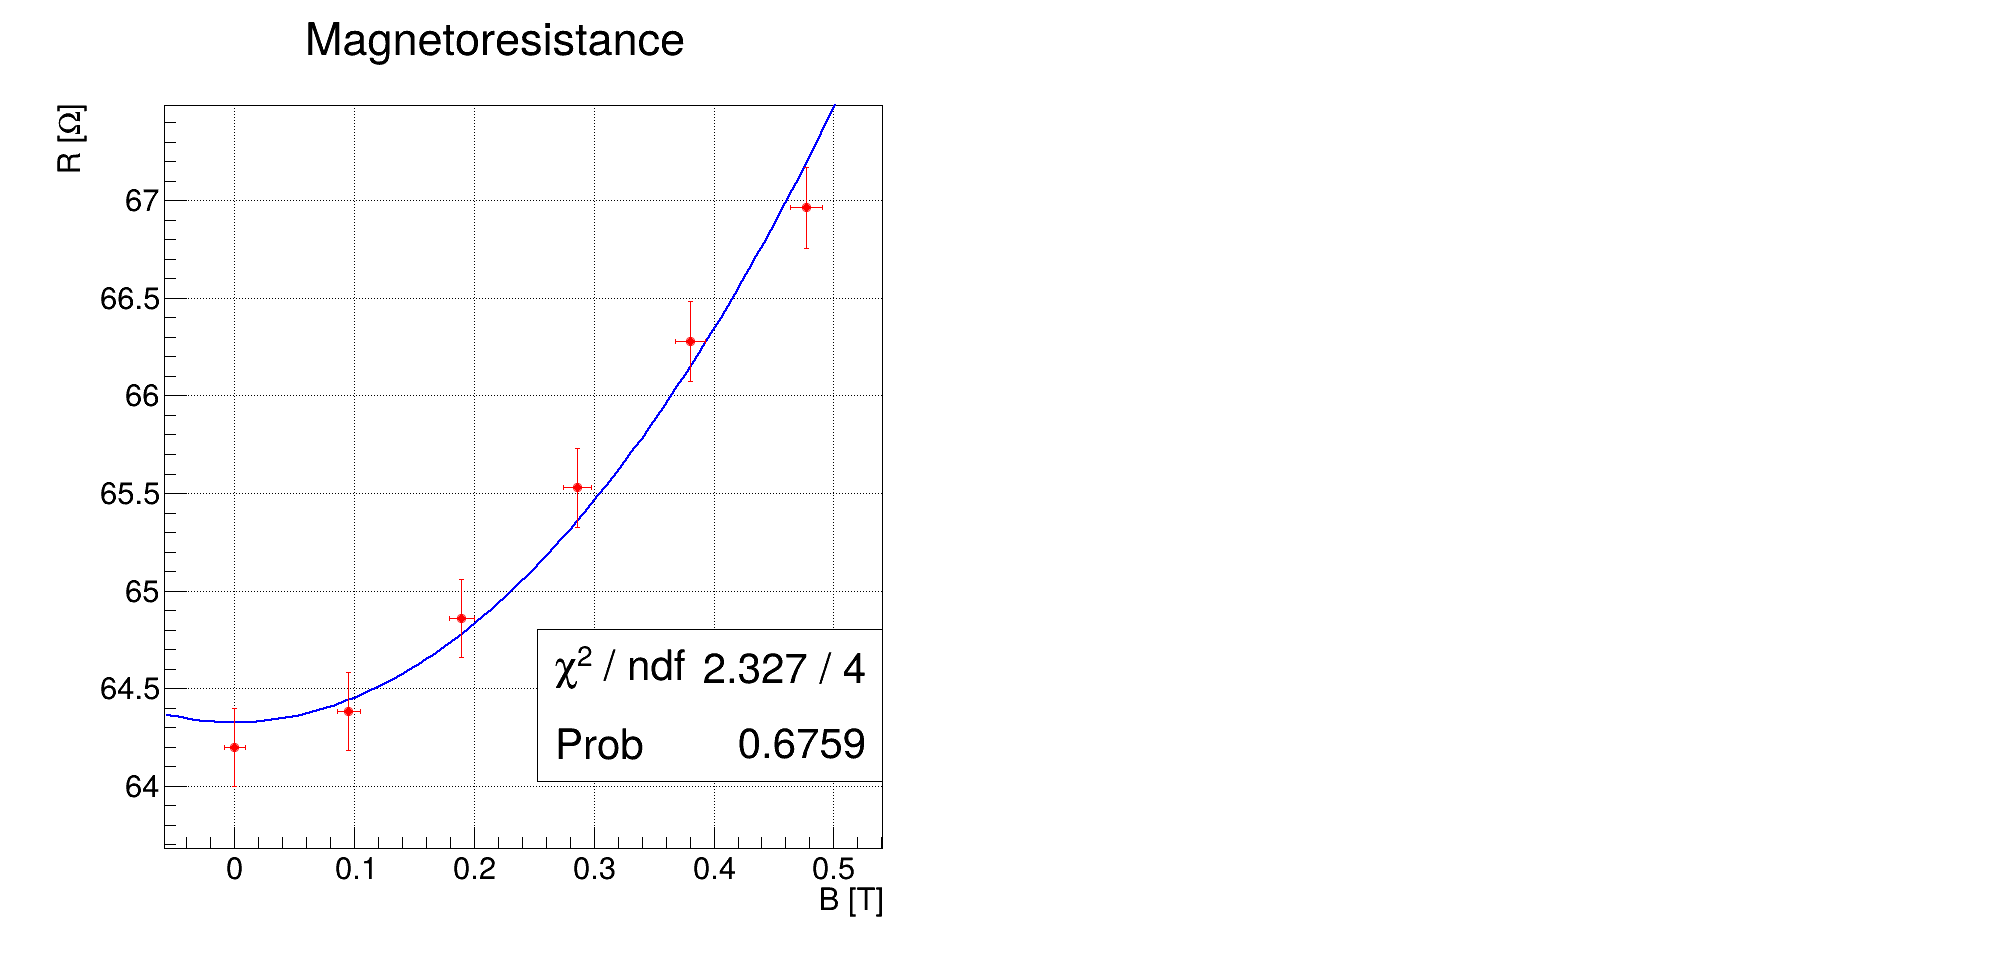
\includegraphics[width=0.85\textwidth]{./figs/magnetoresistance.png}
\caption{Regressione con il modello \cref{eq:magnetoresistance} ai dati in \cref{tab:magnetoresistance}: il risultato del fit è in blu. Le resistenze sono espresse in $ \unit{\ohm} $ mentre i valori di campo magnetico sono stati convertiti in $ \unit{T} $.}
\label{fig:magnetoresistance}
\end{figure}

\begin{figure}
\centering
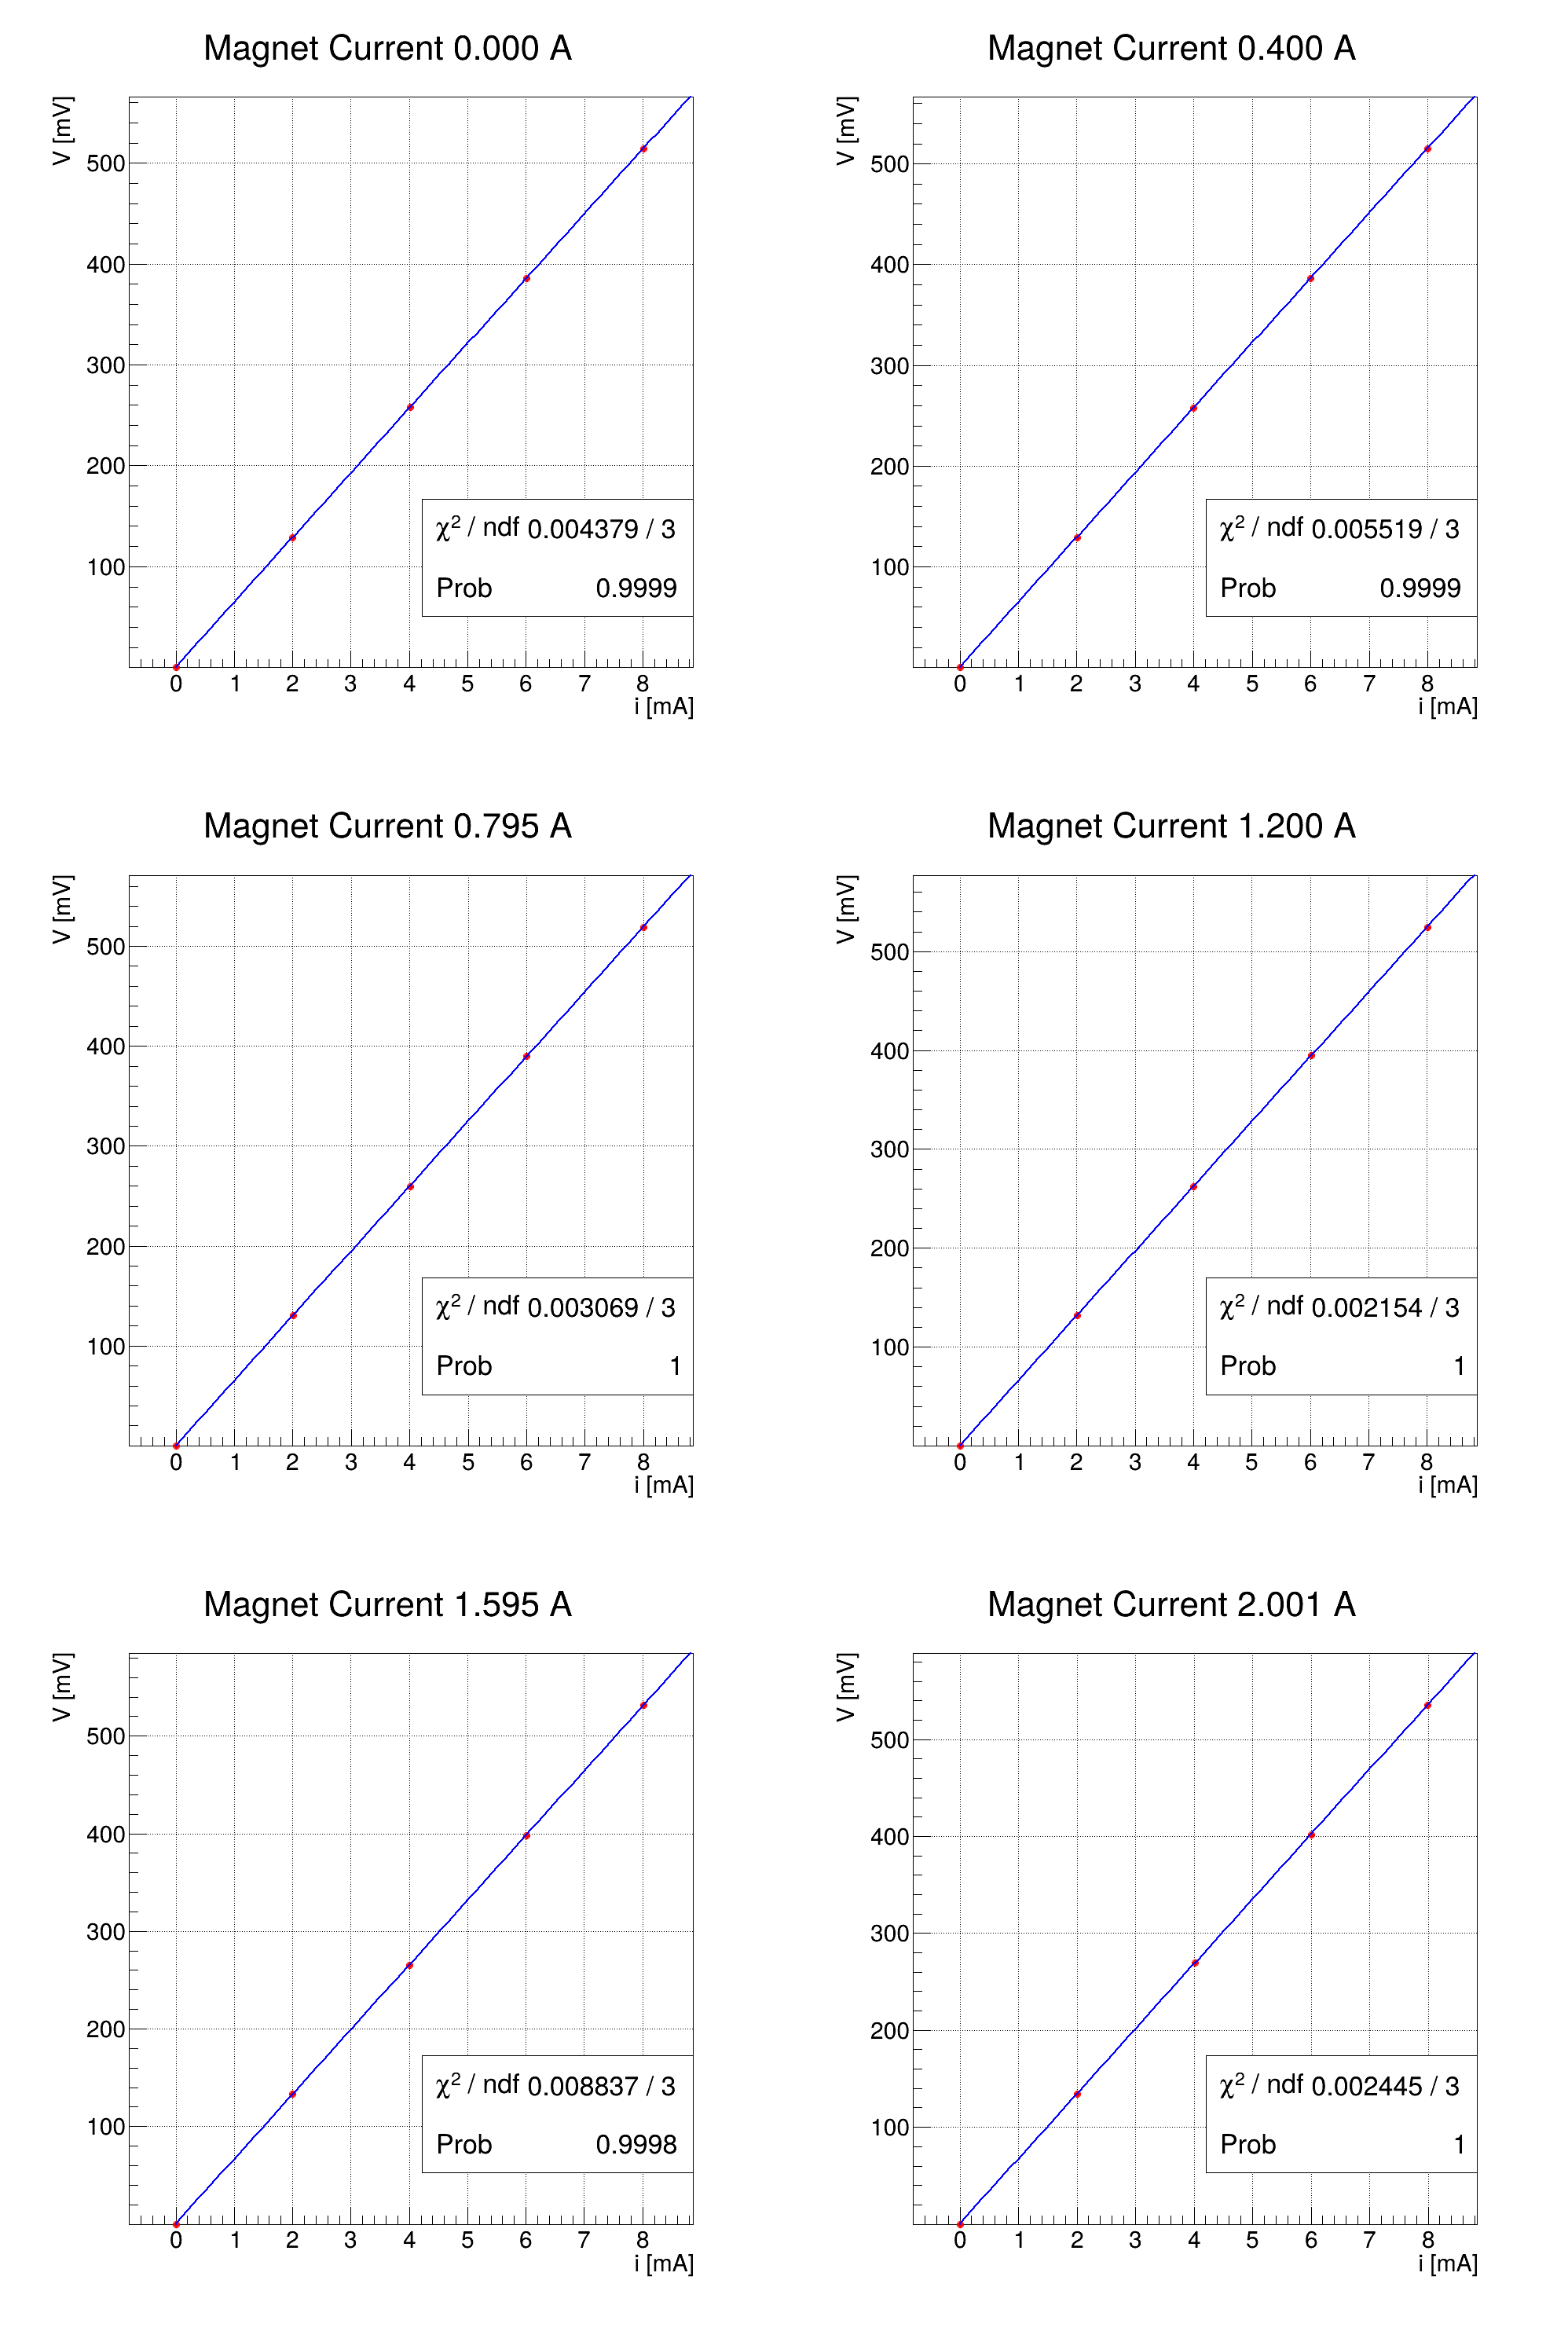
\includegraphics[width=0.85\textwidth]{./figs/resistanceB.png}
\caption{Regressioni lineari alle caratteristiche $ V(I) $ (tensioni in $ \unit{mV} $ e correnti in $ \unit{mA} $) del germanio al variare del campo magnetico esterno (controllato dalla ``magnet current'' nel titolo): i parametri risultato dei fit sono raccolti in \cref{tab:magnetoresistance} associati ai valori di $ B $ corrispondenti.}
\label{fig:IV-Bvaries}
\end{figure}

\subsection{Compatibilità con $ \mu $}

Quindi usando il modello:
\begin{equation}
R = b + aB^2
\end{equation}
per fare una regressione alle resistenze stimate in \cref{tab:magnetoresistance} contro i campi magnetici $ B $, troviamo (in \cref{fig:magnetoresistance}):
\begin{equation}
b = (64.33 \pm 0.12) \unit{\ohm} \qquad a = (12.6 \pm 1.2) \unit{\ohm / T^2}
\end{equation}
da cui allora per confronto con l'\cref{eq:magnetoresistance}:\footnote{Stiamo trascurando la covarianza tra i parametri del fit nella propagazione dell'errore per la stima di $ \mu $.}
\begin{equation}
\mu = (0.44 \pm 0.02) \unit{m^2 / V \cdot s}
\end{equation}
che non è compatibile con l'altra stima che ne abbiamo dato.
